\documentclass[10pt]{article}
\usepackage{icmlko}

\icmlmeta{IP 파운데이션 월드모델}{122}{눈금을 고쳐도 모형은 안 좋아진다}{세 출처를 정직한 라벨로 바꾸니 팝업만 $+$0.0104(보류)이고 나머지 여섯은 $-$0.0018 --- 효과의 전부가 부풀림이 가장 컸던 게임 하나에서 온다}

\begin{document}

\twocolumn[
\icmlheader

\begin{abstract}
노트 121이 관측만 하고 남긴 것을 검정했다 --- 세 출처(세계애니 · 만화 · 게임)의
라벨을 다른 플랫폼 것으로 바꾸면 팝업이 오르는가. 라벨이 바뀐 셋은 대상으로
쓰면 정의가 달라지므로 \textbf{라벨이 안 바뀐 일곱만 대상}으로 뒀다.
\textbf{팝업은 $+$0.0104 오르는데 씨앗 넷 전부 보류}다(구간
$-$0.040$\sim+$0.038). \textbf{나머지 여섯은 $-$0.0018}이다. 부분집합 일곱을
다 돌리니 원인이 하나로 좁혀진다 --- \textbf{게임 하나가 효과의 전부}다.
게임만 바꿔도 $+$0.0100이고 세계애니만 바꾸면 오히려 $-$0.0044다. 게임은
노트 120에서 부풀림이 가장 컸던 도메인이다(38\%, 다른 둘은 21 · 23\%).
\textbf{그래서 이 눈금 이야기(노트 117--122)가 닫힌다.} 여섯 노트에 걸쳐
누수를 잡고(117) 다른 플랫폼을 붙이고(118) 정합을 재고(119 · 120) 법칙을
다시 쟀는데(121), \textbf{측정은 바로잡혔지만 모형은 안 좋아졌다.}
이 프로젝트에서 ``원리적으로 옳은 쪽이 지는'' \textbf{일곱째 사례}다
(노트 40 · 48 · 85--88 · 103 · 105 · 114, 그리고 여기). 다만 이번 것은
빈손이 아니다 --- \textbf{수치를 못 올렸지만 수치의 뜻을 바꿨다.} 팝업의
$+$0.4391은 다른 도메인의 $+$0.54와 견줄 수 없는 값이었고, 정직한 눈금에서
팝업은 열 중 셋째다(노트 120).
\end{abstract}
]

\begin{figure*}[t]
\centering
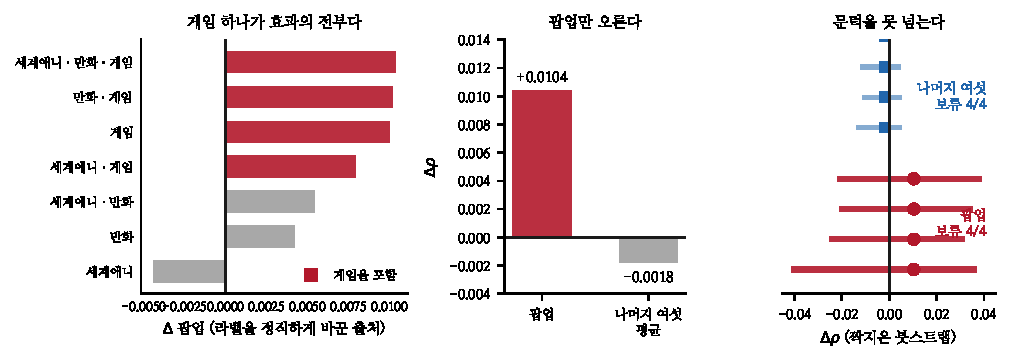
\includegraphics[width=\textwidth]{figs/sf.pdf}
\caption{왼쪽 --- 게임 하나가 효과의 전부다. 가운데 --- 팝업만 오른다.
오른쪽 --- 문턱을 못 넘는다.}
\end{figure*}

\section{부분집합 일곱을 다 돌렸다}

\begin{table}[t]
\centering\tsize
\caption{어느 출처의 라벨을 정직하게 바꾸나. 대상은 라벨이 안 바뀐 일곱.}
\begin{tabular}{lrr}
\toprule
바꾼 출처 & $\Delta$팝업 & $\Delta$나머지 여섯 \\
\midrule
세계애니 & $-$0.0044 & $-$0.0015 \\
만화 & $+$0.0042 & $-$0.0002 \\
\textbf{게임} & \textbf{$+$0.0100} & $-$0.0010 \\
\midrule
세계애니 · 만화 & $+$0.0054 & $+$0.0007 \\
세계애니 · 게임 & $+$0.0079 & $-$0.0017 \\
만화 · 게임 & $+$0.0102 & $-$0.0018 \\
\textbf{셋 다} & \textbf{$+$0.0104} & $-$0.0018 \\
\bottomrule
\end{tabular}
\end{table}

\claimx{\textbf{게임 하나가 효과의 전부다.} 게임만 바꿔도 $+$0.0100이고 셋 다
바꿔도 $+$0.0104다. 세계애니만 바꾸면 오히려 $-$0.0044다. 게임은 노트 120에서
부풀림이 가장 컸던 도메인이다(38\% 대 21 · 23\%).}{셋뿐이라 ``부풀림이 클수록
효과가 크다''를 말할 수 없다 --- 만화(21\%)가 세계애니(23\%)보다 큰 효과를
낸다. 게임이 다른 이유는 부풀림 말고도 있을 수 있다.}

\section{문턱을 못 넘는다}

\begin{table}[t]
\centering\tsize
\caption{셋 다 정직하게. 씨앗 넷 · 짝지은 붓스트랩 100회.}
\begin{tabular}{lrl}
\toprule
& $\Delta$ & 95\% 구간 \\
\midrule
팝업 & $+$0.0104 & $-$0.0401 $\sim$ $+$0.0356 \\
& & $-$0.0242 $\sim$ $+$0.0307 \\
& & $-$0.0200 $\sim$ $+$0.0341 \\
& & $-$0.0207 $\sim$ $+$0.0379 \\
나머지 여섯 & $-$0.0018 & 보류 4/4 \\
\midrule
\multicolumn{3}{l}{\textbf{보류 4/4 --- 채택하지 않는다}} \\
\bottomrule
\end{tabular}
\end{table}

\claimx{\textbf{출처를 정직하게 바꾸는 것이 모형을 좋게 하지 않는다.} 팝업이
$+$0.0104 오르지만 씨앗 넷 다 보류이고, 나머지 여섯은 $-$0.0018로 오히려
미세하게 나쁘다.}{팝업 구간이 $\pm$0.035로 넓다. $n{=}75$ 의 한계이고, 이
크기의 효과를 이 표본으로 가를 수 없다(노트 92).}

\section{눈금 이야기가 닫힌다}

\begin{table}[t]
\centering\tsize
\caption{노트 117--122가 한 것.}
\begin{tabular}{ll}
\toprule
117 & 누수를 잡고 두 겹 가드를 넣었다 \\
118 & 다른 플랫폼(Kitsu)을 붙였다 --- 질은 $\rho{=}+$0.969 \\
119 & 자기 $\rho$ 의 23\%가 같은 플랫폼 정합 \\
120 & 세 도메인에서 21$\sim$38\% 확인, 팝업이 셋째로 \\
121 & 법칙 1은 서고 법칙 2는 반토막 \\
\textbf{122} & \textbf{그런데 모형은 안 좋아진다} \\
\bottomrule
\end{tabular}
\end{table}

\claimx{여섯 노트에 걸쳐 \textbf{측정은 바로잡혔지만 모형은 안 좋아졌다.}
``원리적으로 옳은 쪽이 지는'' 일곱째 사례다(노트 40 · 48 · 85--88 · 103 ·
105 · 114).}{그렇다고 되돌릴 것도 없다 --- 라벨을 안 바꿨고 바꾸지도 않는다.
이 여섯 노트는 \emph{설정}이 아니라 \emph{해석}을 고쳤다.}

\begin{quote}\fontsize{9.5}{11.5}\selectfont
\textbf{다만 이번 것은 빈손이 아니다.} 수치를 못 올렸지만 \textbf{수치의 뜻을
바꿨다.} 팝업의 $+$0.4391은 다른 도메인의 $+$0.54와 견줄 수 있는 값이 아니었고
--- 저쪽은 축과 라벨이 같은 API 에서 나와 21$\sim$38\% 부풀려져 있었다 ---
정직한 눈금에서 팝업은 열 중 셋째다. \textbf{지난 열다섯 노트가 ``팝업이
왜 이렇게 낮은가''를 물었는데, 질문 자체가 틀렸다.}
\end{quote}

\section{한계}

\begin{itemize}[leftmargin=1.1em,itemsep=0.15em]
\item \textbf{채택할 것이 없다.} 팝업 $+$0.0104가 보류 4/4다.
\item 부분집합 일곱에서 게임 하나가 지렛대인데 이유를 모른다.
\item 남은 다섯 도메인(모바일 · 웹툰 · 도서 · 펀딩 · 애니)은 정직한 라벨을
      아직 못 구했다 --- 노트 120의 순위표 절반이 추정이다.
\item 라벨을 바꾸면 표본이 조금 준다(만화 1,789 $\to$ 1,596). 표본 변화가
      섞여 있다.
\item 팝업 구간 $\pm$0.035. 이 크기의 효과를 $n{=}75$ 로 못 가른다.
\end{itemize}

\section{다음}

\begin{enumerate}[leftmargin=1.3em,itemsep=0.15em]
\item \textbf{눈금 이야기를 접고 제품으로 돌아간다} --- 여섯 노트가 해석을
      고쳤고 성능은 그대로다. \texttt{state/score.py} 의 자기 검사와 노트 91의
      도구 순위표를 정직한 눈금으로 다시 내 \textbf{문서만 고친다.}
\item \textbf{게임이 왜 다른가} --- 부분집합 실험의 유일한 미해결.
\item \textbf{팝업 레코드} --- 열여섯 노트가 같은 곳을 가리킨다. 이제
      ``팝업이 낮아서''가 아니라 ``구간이 넓어서''다. \textbf{모으는 절차를
      설계할 때가 됐다.}
\item 남은 다섯의 정직한 라벨.
\end{enumerate}

\vspace{0.6em}
\hrule height 0.3pt
\vspace{0.5em}
{\footnotesize
\textbf{참고문헌}\\[0.3em]
Campbell, D. T., Fiske, D. W. (1959). Convergent and discriminant validation by
the multitrait-multimethod matrix. \emph{Psychological Bulletin}, 56(2), 81--105.\\[0.15em]
Lord, F. M., Novick, M. R. (1968). \emph{Statistical Theories of Mental Test
Scores}. Addison-Wesley.\\[0.15em]
Efron, B., Tibshirani, R. J. (1993). \emph{An Introduction to the Bootstrap}.
Chapman \& Hall.\\[0.15em]
Varoquaux, G. (2018). Cross-validation failure: small sample sizes lead to large
error bars. \emph{NeuroImage}, 180, 68--77.\\[0.15em]
Ben-David, S. et al. (2010). A theory of learning from different domains.
\emph{Machine Learning}, 79(1--2), 151--175.
}

\end{document}
